% \documentclass[11pt]{acm_proc_article-sp}
\documentclass[11pt, twocolumn]{article}
\setlength{\columnsep}{35pt}
\usepackage[left=.8in, right=.8in, top=1.1in, bottom=1.1in]{geometry}


\usepackage{wrapfig}
\usepackage{tikz, alex, url, mu}
\usetikzlibrary{arrows,shapes,snakes,automata,backgrounds,petri}
\tikzset{>=stealth}

\usepackage{algorithm}
\usepackage{algorithmic}

\title{Quilting for Distributed Machine Learning System}

\author{Mu Li \quad Jinliang Wei\\ Computer Science Department
  \\Carnegie Mellon University\\
  5000 Forbes Ave., Pittsburgh, PA, 15213\\
\{muli, jingliangw\}@cs.cmu.edu}

\begin{document}
\maketitle

\begin{abstract}
  Distributed machine learning applications produce a huge amount of network
  traffic. However, network bandwidth is one of the most scarce resources in
  data centers.  In this paper we propose QuiltDB, which is a distributed
  database execution engine optimized for network topology. QuiltDB trades off
  latency for high bandwidth. It executes as a discrete streaming system and
  allow users to specify desirable network topologies. We evaluate this system
  on several machine learning applications with real datasets\footnote{C++ codes
    are available at \url{https://github.com/jinliangwei/quiltdb/}}.
\end{abstract}

\section{Introduction}

In distributed machine learning applications, both data and computations are
partitioned into hundreds or  thousands of machines. Those
worker machines compute local results based on their own part of data. Global solutions
are then obtained via synchronization \cite{AhmSheNarJosSmo13,
  HoCipCuiLeeetal13,Lietal13,DeaCorMonCheetal12,GonLowGuBicetal12,CheSonBaiLinetal11}.

Synchronization, including data communication and waiting the slowest machine, is typically
the most expensive operation, because of the limited network bandwidth and highly
variant machine performances. Recently, asynchronous computation is proposed
to hide this synchronization cost. However, they assume the network has fully
bisection bandwidth \cite{AsuSmyWel08,SmoNar10,AhmSheNarJosSmo13,Lietal13}.

On practice, the real data center network has special topologies. One common
topology is the multi-rooted tree, where  machines are first grouped by racks,
and these racks are then connected by
end of row and core switches. The network bandwidth in this tree is not
uniform. Typically bandwidth within a leaf node (a rack) is usually much larger
than the others~\cite{AlFLouVah08, BarHol09}.

Machine learning applications should consider the network topology, because of
its huge amount of data communication volume and iterative nature. A proper
communication pattern could reduce the network congestion, e.g.~core switches,
and therefore reduce the waiting time. In addition,
if the communication forms a simple pattern, such as a ring or a star, then it
is much easier to improve the physical network according this to pattern than
improve the overall point-to-point bandwidth.

On this paper, we propose a database execute engine, QuiltDB, which mapping
machine learning applications into network topologies. Key features of this
system includes,

\begin{itemize*}
\item Grid data partition. Traditional databases uses either vertical or
  horizontal partitions. However, a grid partition could reduce the network
  traffic volume if the training data is near square, namely the number of
  instances and features are on the same scale.
\item Model machine learning applications using the
  primal-dual approach. The primal-dual decomposition fits into the grid
  partition in nature, where the primal variables are shared horizontally, while
  the dual variables are communicated vertically.
\item Allow use-defined network topology. QuiltDB allows user to configure the
  logical network connection.
\item A discrete streaming system. QuiltDB is implemented as a discrete
  streaming system. Different to previous system, QuiltDB merging keys (similar
  to reduce) at every node, and also allow loop exists in the stream.
\end{itemize*}

\section{Network Topologies}
\label{sec:network-topologies}

Several network topologies have been proposed by HPC community, including grid,
hyper-cube, buffer-fly, etc. Algorithms are then mapped into network topology to
maximize the communication efficiency. On the other hand, cloud computing
typically adopts
tree-like structures, which aims to approximate an uniform all-to-all connection
and provide fault tolerance and elastic scalability.

\subsection{Grid Communication}

Grid is the one of the simplest communication pattern, which is shown in
Figure~\ref{fig:grid2} \cite{DeeBlyGilKesetal04, FosZhaRaiLu08}. Machines are connected both vertically and
horizontally. Each node only communicates with its vertical and horizontal
neighbors. In physical, neighbors nodes are directly connected, or sitting
near-by each other, e.g.~within the same rack,  so that high network bandwidth
between neighbor nodes are guaranteed. One advantage of grid communication is
the low cost of building its network. If each machine have hour network ports,
then expensive switches are not even necessary. On the other hand, this
communication pattern explicitly uses network space locality, so it is also
suitable for high network traffic volume applications, if the physical network
is not good enough.

However, if two nodes are not connected directly, then they need to communicate via
other nodes. This path is possible long,  so the delay might be high. For
example, in a $n\times n$ grid, and denote by $\tau$ the RTT  between
two neighbor nodes, then the RTT between the left-upper corner node and
right-bottom node is $2n\tau$.

\begin{figure}[th!]
  \centering
  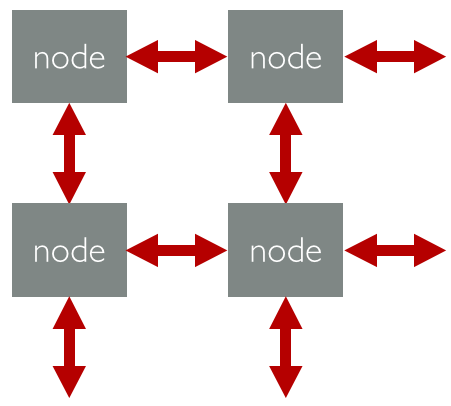
\includegraphics[width=.45\textwidth]{fig/grid}
  \caption{Grid communication. Each machine only communicates with its 4
    neighbors, and typically enjoys high network bandwidth. However, the network
  delay might be large if two nodes are far away.}
  \label{fig:grid2}
\end{figure}

\subsection{Data Center Topologies}

The real network in a data
center nowadays usually has a tree-like structure. Machines are first connected
by the top of rack switch and typically enjoy high bandwidth if two machines
shared the same switch. Racks are then connected by end of row and core
switches. Due to the large number of racks (10---100), cost, energy consuming,
and cabling complexity, it is hard to have full bisection bandwidth. A typical
oversubscription ratio is between 2:1 to 8:1, which means the average bandwidth
between two racks is typically much less than the one within a
rack~\cite{AlFLouVah08, BarHol09}.

The grid communication is somewhat too restrictive in the data center environment. However, the all-to-all
communication places too much burden to end of row and core switches. A hybrid
communication, shown in Figure~\ref{fig:rack}, combines the advantages of the
previous two patterns. Due to the high
inner switch bandwidth, machines in the same rack can communicate to each other
in a flexible way. However, we restrict the connections crossing racks. In other
words, we first place all racks sides by sides, then we let all machines
communicate to their horizontal neighbors only.


\begin{figure}[th!]
  \centering
  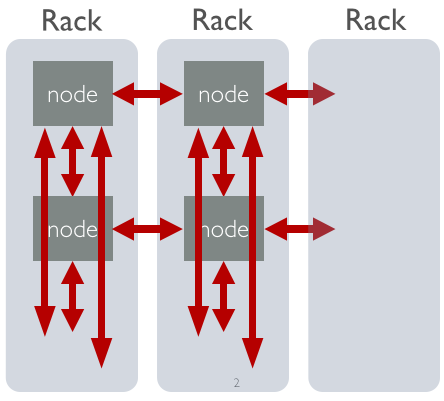
\includegraphics[width=.45\textwidth]{fig/rack}
  \caption{Flexible connections within a rack, while restrict the communication
    between racks. }
  \label{fig:rack}
\end{figure}

\section{Machine Learning Applications}

In this section, we describe several machine learning applications which fits
into the communication pattern we discussed on Section
\ref{sec:network-topologies}.

\subsection{Data Partition}

On a typical distributed machine learning application, both data and shared
parameters are partitioned into a group of machines.
Different partitioning scheme requires different amount of data to be
communicated. For example, consider the following iterative matrix
multiplications, which is a typical machine learning workload:
\begin{align*}
w &= X u \\
u &= X^T w,
\end{align*}
where $X$ is a gigantic data matrix and $u$ and $w$ are two vectors.

Given a $n$-by-$m$ matrix $X$, we want to divide the matrix into $p$ machines
while minimizing the amount of data to be communicated in each iteration.

If we cut the matrix into $a$ rows and $b$ columns, then the minimal data
communication is

\begin{equation}
  r  am +  c bn
  \label{eq:total-traffic}
\end{equation}
where $r,c \in [0,1]$ are coefficient depending on the sparsity of the
matrix. They should be a function as $a$ and $b$, but now we consider it as a
constant to simply the calculation.

Note that $ab=p$, then (\ref{eq:total-traffic}) get minimize value when
$a = \rbr{ \frac{cn}{rm} }^{\frac{1}{2}}\sqrt{p}$. That is, if $cn \gg rm$, we
should choose partition scheme 1, if $rm \gg cn$, we should use scheme 2, while
if $rm \approx cn$, the even partition scheme 3 is a better choice.

\begin{figure*}[th!]
  \centering
\begin{tikzpicture}[scale=.8]
  \draw [fill=set12!60](0,0) rectangle (4,1)
  rectangle (0,2) rectangle (4,3) rectangle (0,4);
  \draw[xshift=6cm, fill=set11!60] (0,0) rectangle (1,4) rectangle (2,0) rectangle (3,4)
  rectangle (4,0);
  \draw[xshift=12cm, fill=set13!60] (0,0) rectangle (2,2) rectangle (0,4);
  \draw[xshift=14cm, fill=set13!60] (0,0) rectangle (2,2) rectangle (0,4);
\end{tikzpicture}
  \caption{partition scheme 1 to 3: $a=4,b=1$, $a=1,b=4$, and $a=2,b=2$}
\end{figure*}

\subsection{Pagerank}
\label{sec:pagerank}

Given adjacent matrix $X$, where $X_{ij} = 1 $ if and only if webpage $i$ cites
$j$. Denote by $D=\textrm{diag}{\sum_i X_{i1}, \ldots, \sum_{i=1} X_{in}}$ the diagnal
adjacent matrix, then pagerank can be solved by.
\begin{equation}
  w = \alpha X^T D^{-1} w + (1-\alpha)\frac{1}{n}
\end{equation}

\begin{figure}[th!]
  \centering
  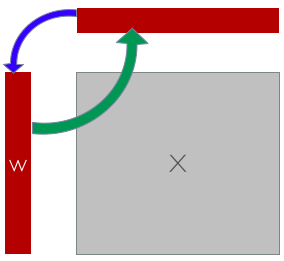
\includegraphics[width=.4\textwidth]{fig/pr}
  \caption{Pagerank, we explicit decompose the workload into two step. First
    compute a new value of $w$ (green arrow), and then update $w$ (blue arrow).}
  \label{fig:pr}
\end{figure}

The workload is summarized in Figure~\ref{fig:pr}. It is convenient to view the
updating as two steps, the
first step compute the new value of $w$, and then update $w$. To extend pagerank
into a distributed algorithm, we consider the grid data partition. Then each
machine also execute the computing and then updating steps. The only difference
is that updating involves network communications.

Figure~\ref{fig:dist_pr} shows an distributed implementation using the grid
communication. While Figure~\ref{fig:dist_pr2} shows a version using the
tree-ring topology. In other words, each rack get a group of columns of $X$. All
machines in a rack form a tree, one particular machine is selected as a
root. This root gathers all updates within the rack and then propagates to its
neighbor rack.

\begin{figure*}[th!]
  \centering
  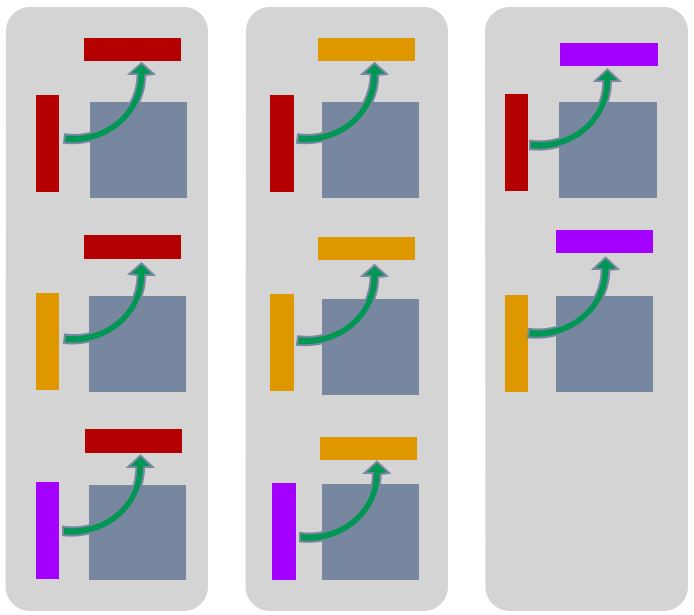
\includegraphics[width=.4\textwidth]{fig/compute} \hspace{4ex}
  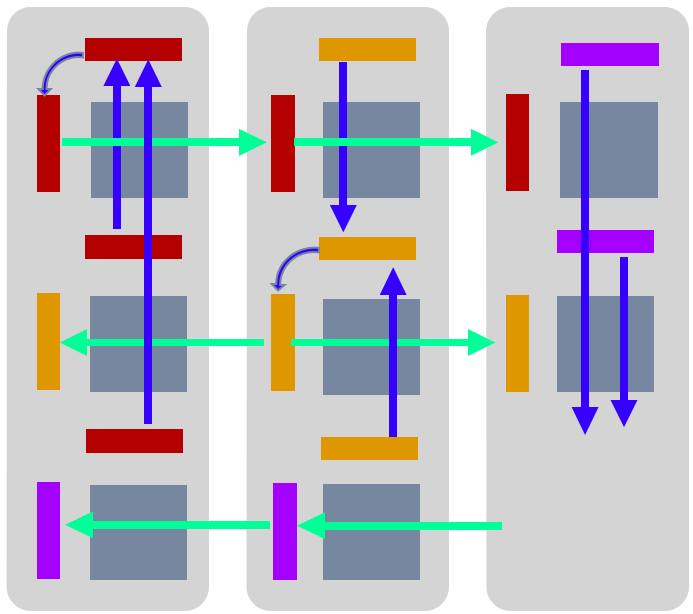
\includegraphics[width=.4\textwidth]{fig/update}
  \caption{Distributed Pagerank using a hybrid topology. Left: compute; right update}
  \label{fig:dist_pr}
\end{figure*}


\begin{algorithm}[tb]
  \caption{Distributed Pagerank with Grid topology}
  \label{algo:pr}
  \begin{algorithmic}[1]
    \REQUIRE Assume $n\times m$ machines, grid partition of the $\ell \times \ell$
    adjacent matrix. machine
    $m_{i,j}$  gets data block $X_{i,j}$, and weight block $w_i$.
%    \ENSURE
    \FOR [asynchronous] {all machines in parallel}
    \FOR {$t=0,\ldots,T$}
    \STATE compute $u_j \gets \alpha X_{i,j}^T D_{i,j}^{-1} w_i +
    (1-\alpha)\frac{1}{\ell m}$
    \IF { $i=j$ }
    \STATE $w_i \gets u_j$
    \STATE send $w_i$ to machine $m_{i+1,i}$
    \ELSE
    \STATE send $u_j$ to machine $m_{i,j+1}$
    \ENDIF
    \ENDFOR
    \ENDFOR
  \end{algorithmic}
\end{algorithm}


\begin{algorithm}[tb]
  \caption{Distributed Pagerank with Tree-ring topology}
  \label{algo:pr2}
  \begin{algorithmic}[1]
    \REQUIRE Assume $n\times m$ machines, grid partition of the $\ell \times \ell$
    adjacent matrix. Machine
    $m_{i,j}$  gets data block $X_{i,j}$, and weight block $w_i$.
%    \ENSURE
    \FOR [asynchronous] {all machines in parallel}
    \FOR {$t=0,\ldots,T$}
    \STATE compute $u_j \gets \alpha X_{i,j}^T D_{i,j}^{-1} w_i + (1-\alpha)\frac{1}{nm}$
    \IF { $i=j$ }
    \STATE $w_i \gets u_j$
    \STATE send $w_i$ to machine $m_{i+1,i}$
    \ELSE
    \STATE send $u_j$ to machine $m_{i,i}$
    \ENDIF
    \ENDFOR
    \ENDFOR
  \end{algorithmic}
\end{algorithm}

\subsection{Loss minimization}

Loss minimization solves the following optimization problem:
\begin{equation}
  \min_w F(w) = \sum_{i=1}^{n} f(\langle x_i, w\rangle, y_i) + \lambda r(w)
\end{equation}

Let consider the gradient descent as an example to solve this problem. On each
iteration, gradient descent compute the gradients based on the current weight $w$.

\begin{align*}
  \partial F(w) &= \partial \sum_{i=1}^{n}  f(\langle x_i, w\rangle, y_i) +
  \lambda r(w) \\
  &= \sum_{i=1}^{n} x_i \partial f(\langle x_i, w\rangle, y_i) +
  \lambda \partial r(w)
\end{align*}

A new weight is computed as $w' = w - \eta \partial F(w)$, where $\eta$ is the
learning rate. This algorithm fits into our system by the primal-dual
viewpoint. The weight $w$ is the primal
variable, and
\begin{equation}
  u = X w
\end{equation}
is treat as the dual variables.
Then the gradient descent computes and updates
the prime and dual alternatively. Furthermore, $\partial f$ is typically a
scalar function with respect to the dual variables and labels. For square loss,
we have
\begin{align*}
  f(u,y) & = \frac{1}{2} \|u-y\|^2, \\
  \partial f(u,y) &= u-y \\
\end{align*}
    and for logistic loss:
  \begin{align*}
f(u,y) & = \log(1+\exp(-y u))  \\
  \partial f(u,y) &= \frac{1}{1 + y\exp(-yu)}
\end{align*}



\begin{algorithm}[tb]
  \caption{Distributed Pagerank with Tree-ring topology}
  \label{algo:loss}
  \begin{algorithmic}[1]
    \REQUIRE Assume $n \times m$ machines, grid partition of data. machine
    $m_{i,j}$  gets data block $X_{i,j}$, and weight block $w_j$.
%    \ENSURE
    \FOR [asynchronous] {all machines in parallel}
    \FOR {$t=0,\ldots,T$}
    \STATE compute dual variable $u_i \gets X_{i,j} w_j$
    \IF {$i=j$}
    \STATE machine $m_{i,i}$ gathers all $u_i$ from machine $m_{i,1}, \ldots,
    m_{i,n}$. We may ignore the results of lowest machine or allow delayed
    results to improve the performance of this aggregator
    \STATE broadcast $\partial f(u_i, y_i)$
    \ELSE
    \STATE send $u_i$ to machine $m_{i,i}$
    \ENDIF
    \STATE compute delta $\delta_j = X_{i,j}^T \partial +
    \frac{\lambda}{n} \partial r(w)$
    \STATE send $\delta_j$ to machine $m_{i+1,j}$
    \STATE apply delta $w \gets w - \eta \delta_j$
    \ENDFOR
    \ENDFOR
  \end{algorithmic}
\end{algorithm}

\section{Programming Model}

QuiltDB provides a distributed in-memory key-value store for accessing shared
data. Key-value pairs are organized as tables and tables are shared among
nodes along the same \emph{oplog propagation path}. Updates to shared key-value
pairs are propagated along {oplog propagation path}s. Typically, a QuiltDB
process occupies a physical node and it
consists of multiple \emph{logical node}s. Each {logical node} may
participate in one {oplog propagation path}. That is, a {logical node}
receives updates generated by other nodes along the path and forwards them to
its downstream node along with its own updates. With multiple {logical
node}s, a QuiltDB process may participate in multiple {oplog propagation
path}s. With the help of callback functions (Section~\ref{sec:callback})
participating in multiple {oplog propagation path}s
allows a QuiltDB process to act as hub to relay updates along one path to
another path.

When using QuiltDB, the user needs to configure the network topology
({oplog propagation path}s). QuiltDB lets user provide information of
each {logical node} and configure the network topology by simply choosing
the proper downstream node for each {logical node}. A {logical node}
may have at most one downstream node, while it may have many upstream nodes.
Having multiple upstream nodes allows a single node to aggregate updates from
multiple sources. Restricting a {logical node} to have only one downstream
node allows QuiltDB to support cyclic {oplog propagation path}s with simple
oplog deduplicatoin mechanism (see Section~\ref{sec:cyclic-path}).


\begin{figure}[th!]

%\begin{verbatim}
\begin{lstlisting}
class Table{
  template<typename ValueType>
  ValueType Get(int64_t _key);

  template<typename ValueType>
  void Inc(int64_t _key,
           ValueType _delta);
};

typedef int (*ValueAddFunc) (
  uint8_t *v1,
  const uint8_t *v2,
  int32_t size);
typedef int (*ValueSubFunc) (
  uint8_t *v1,
  const uint8_t *v2,
  int32_t size);
\end{lstlisting}
%\end{verbatim}
\caption{Semantics of QuiltDB table APIs and the addition and subtraction
  functions}
\label{fig:table-api}
\end{figure}

\subsection{Key-Value Interface}

As mentioned above, the data stored in QuiltDB are key-value pairs organized
as tables. Values are treated as byte array internally and values stored in one
table are required to have the same size. Supporting multiple tables allows
QuiltDB to support different types of data.

QuiltDB requires the value type to support two operations, \emph{addition} and
\emph{subtraction}. In order to support update aggregation, {addition} must
 be commutative and associative. For numerical types,  the meaning of
{addition} and {substraction} are straightforward. The interface of
QuiltDB tables and the semantics of addition and subtractions are shown in
Figure~\ref{fig:table-api}.

The only write operation supported by the key-value storage is INC which takes
in a delta and apply the delta to a value via {addition}.

\subsection{Callback Functions}
\label{sec:callback}

In most cases, when updates from other nodes are received, they are applied to
local copy of shared data and forwarded to downstream node silently.
However, there are applications that need to be notified upon receiving updates
to perform some special procedure, such as relaying the updates received from
one path to another. For this special case, QuiltDB allows aplication to
register a callback per table which is executed upon the receipt of updates. As
said in Section~\ref{sec:pagerank}, the callback function is essential to
propagate updates to other ranks.

Application may set proper flags on a table to let QuiltDB perform any
combination of the three actions on received updates:
\begin{enumerate*}
\item apply them on local copy
\item forward them to downstream node
\item execute user callback.
\end{enumerate*}

\subsection{User-defined Topology}

User can define desired network topology by configuration. The configure should
specify the network address of the node, and a single downstream node. A topology could
contain loops.

\begin{figure}[th!]
  \centering
\begin{lstlisting}
NodeConfig:
  - id: 0
    recv-pull-ip: 127.0.0.1
    recv-pull-port: 9999
    recv-push-ip: 127.0.0.1
    recv-push-port: 10000
    num-props: 1
    downstream-id: 2
  - id: 1
    recv-pull-ip: 127.0.0.1
    recv-pull-port: 10001
    recv-push-ip: 127.0.0.1
    recv-push-port: 10002
    num-props: 1
    downstream-id: 3
  - id: 2
    recv-pull-ip: 127.0.0.1
    recv-pull-port: 10003
    recv-push-ip: 127.0.0.1
    recv-push-port: 10004
    num-props: 1
    downstream-id: 0
  - id: 3
    recv-pull-ip: 127.0.0.1
    recv-pull-port: 10005
    recv-push-ip: 127.0.0.1
    recv-push-port: 10006
    num-props: 1
    downstream-id: 1
\end{lstlisting}
  \caption{Sample network topology configuration}
\end{figure}

Figure~\ref{fig:topo1} and Figure~\ref{fig:topo2} show some common network
topologies.

\begin{figure*}[th!]
  \centering
  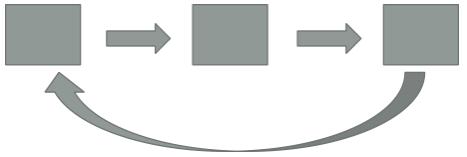
\includegraphics[width=.4\textwidth]{fig/ring}
  \hspace{4ex}
  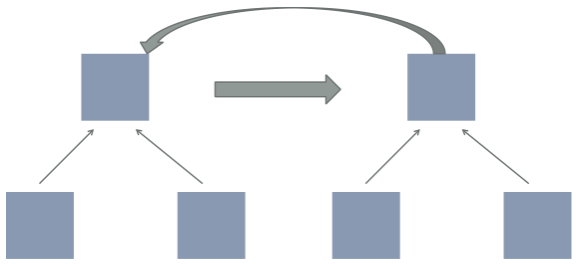
\includegraphics[width=.4\textwidth]{fig/tree}
  \caption{Ring and Tree}
  \label{fig:topo1}
\end{figure*}


\begin{figure*}[th!]
  \centering
  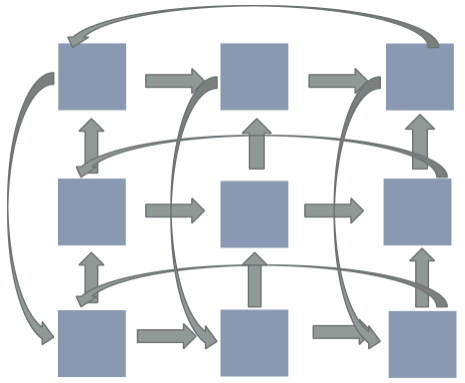
\includegraphics[width=.4\textwidth]{fig/ring_ring}
  \hspace{4ex}
  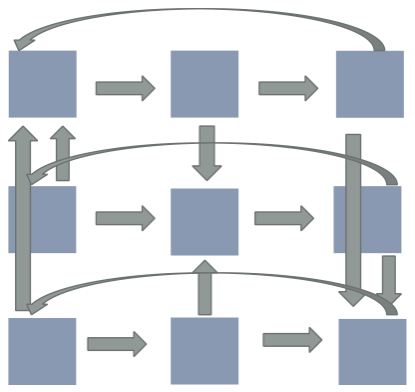
\includegraphics[width=.4\textwidth]{fig/ring_tree}
  \caption{Grid and A combination of ring and tree}
  \label{fig:topo2}
\end{figure*}

\section{Implementation}
In this section, we discuss our system implementation along with techniques to
minimize communication cost.

\begin{figure*}[th!]
  \centering
  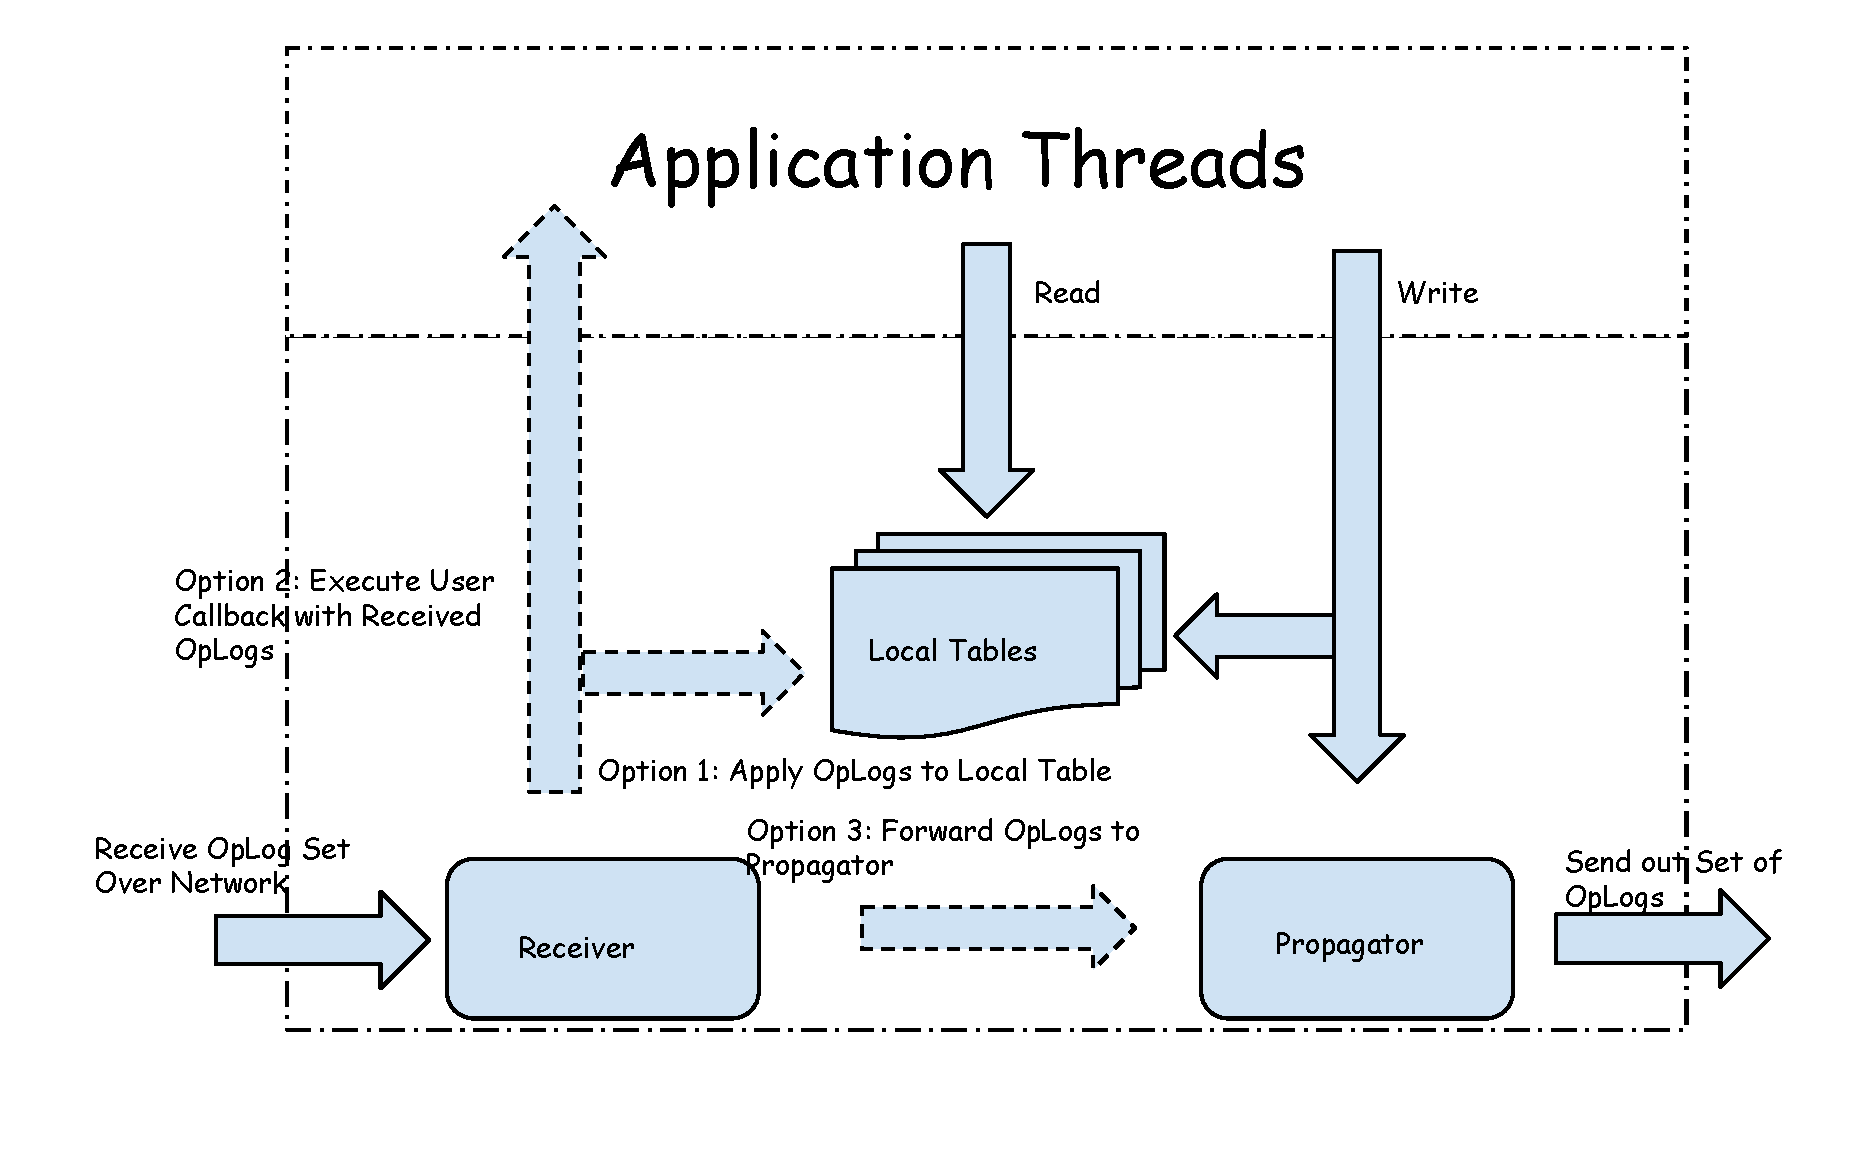
\includegraphics[width=.8\textwidth]{fig/propagator-receiver.pdf}
  \caption{Single Node Architecture}
  \label{fig:prop-recv}
\end{figure*}

\subsection{Propagator-Receiver Pair}

Typically, each physical node runs one QuiltDB process. The architecture of a single
QuiltDB process is visualized in Fig~\ref{fig:prop-recv}.  The QuiltDB process
contains a set of application threads which execute application procedures and
access the distributed paramters via the QuiltDB stub, which consists of one
or multiple \emph{logical node}s.

The core of a QuiltDB \emph{logical nodes} is a paired propagator-receiver
structure. Namely the propagator-receiver pair consists
of a receiver, a propagator and a set of tables registered with this
\emph{logical node}. The \emph{logical node} serves read and write accesses to
key-value pairs, batches and aggregates operation logs for writes and propagate
them to other QuiltDB processes, receives incoming operation logs and act upon
received operation logs appropriately according to corresponding table
configurations. One \emph{logical node} lets the QuiltDB process to participate
in one update propagation path. A QuiltDB stub may contain multiple
\emph{logical node}s and there is no limit on the number of \emph{logical
node}s. Howerver, our current implementation supports up to two \emph{logical
node}s as that suffices the needs of most applications.

As said above, a \emph{logical node} may have multiple tables registered with it.
When application threads read a key via GET(), the value is served directly from
the concurrent hash table. When application threads write a key via INC(), the
operation is applied to the concurrent hash table and a operation log is
appended to the propagator OpLog queue. The propagator thread reads the
operation log from the queue. Instead of sending out the operation log
immediately, the propagator batches operation logs and aggregate them (see
Section~\ref{sec:update-aggreg} for more details) in order to minimize
communication overhead. Batched operation logs are grouped by table ID and are
sent out every $n$ micro-seconds, where $n$ is a user-configurable parameter.

A \emph{logical node} may have at most one \emph{logical node} as its downstream
receiver. A logical node's propagator is connected with the downstream node's
receiver and the aggregated operation logs are sent from propagator to receiver
at the end of each batch interval. Propagators and receivers of the same QuiltDB
process may use different NICs to maximzie network utilization. Upon receiving
a set of updates, the receiver performs actions according to flags set on table
by user application.

\subsection{Update Aggregration and Cyclic Path}
\label{sec:update-aggreg}
\label{sec:cyclic-path}

Since the increment operation on value is commutative and associative, QuiltDB
may aggregrate updates on the same value to reduce the amount of data to be
communicated.

QuiltDB also support cyclic \emph{oplog propagation path}s to minimize
communiation cost. Cyclic \emph{oplog propagation path}s requires QuiltDB to
deduplicate updates as a node may receive its own updates if it is on a cylic
path. When a propagator sends out a set of updates to downstream node, it
notifies the paired receiver first. The paired receiver records the updates
generated at this node then acknowledge the propagator to send out the updates.
Thus when a receiver receives a set of updates, it may check if the set contains
its own updates and remove them before performing other actions upon the
received updates.




\section{Experiments}

\subsection{Setup}

We will evaluate two algorithm. One is pagerank, the other one is logistic
regression, a loss minimization algorithm with logit loss. The latter is still
under developing. We use two large scale real datasets. One is the hyperlink
graph\footnote{\url{http://webdatacommons.org/hyperlinkgraph/}}, which consists
of 3.5 billion web pages and 128 billion hyperlinks. The raw text data is
roughly 1 Terabyte, and consumes around 1 Terabyte memory by storing the page-id
by 64-bit integer. The other one is a Twitter dataset crawled at CMU on the past
4 years. It has around 1 billion of samples and hundreds millions of
features.

We evaluate our system on PDL's cluster Susitna, which has 36 machines in
total. Each machine has 64 AMD cores and 128G memory. All machines are connected
to a single top-rack switch.

We compare our system against two other two systems. One is a standard BSP
model implemented by MPI. The communication is done by AllReduce, which merges
the results via a tree path. The other system is parameter server. It is an
asynchronous machine learning system using a server/client architecture.

\subsection{Planed Experiments}

Ideally we should evaluate our system on a datacenter using hundreds of
machines with even larger datasets, where the network congestion is more
serious. However, we will try Susitna first, because of its better machine
configuration than other PDL clusters. The 40G network bandwidth of Sustina may
be too good for our experiments. We will use tool to limit its
bandwidth. Another PDL cluster under our consideration is Marmort. It owns more
machines than Sustina, but each machine only has two cores and 4G memory, it
makes our implementation more challenge.

One key experiment will be comparing running time versus objective value, under
different network configurations. We expect that MPI is the least efficient
system, because of the synchronous communication. QuiltDB may outperform
parameter server, especially for very large dataset but poor network.


% \appendix
% \section{Acknowledgements}
% The authors would like thank to Alex Smola, Dave Andersen (potentially more...)
% for helpful discussion.

%\bibliography{ref}
\bibliography{../../../bibfile/bibfile}
\bibliographystyle{plain}

\end{document}
